\section{Experimental Results}
\label{sec:eval}
In this section, we evaluate our clustered based image search system.
At the beginning, we introduce the test data and evaluation metrics.
Then, we show four experiments of our system.
The first experiment shows the performance of each key component
of our system: context extraction, representation, and
 the combination of textual and visual information;
The second one gives an end-to-end comparison between our
 approach and the start-of-the-art systems;
The third one illustrates the accuracy of concepts that generated
by our system for each cluster.
The last one shows the efficiency of our system.
%At the end of this section, we show the representative top ranked concept
%lists of some resulting clusters.

%\subsection{Preparation}
%Talk about setup of the experiment, including running environment, selection of parameters, etc.

\subsection{Experiment Setup}
%We prepare two kinds of data set for testing. One is for comparison with other image clustering methods,
%the other is for document clustering. All of the data set can be obtained from internet.

%\textbf{Image Clustering Data:}
We prepare a set of image clustering data from Google Image Search
sorted by relevance.
We select a list of 50 ambiguous queries as shown in \figref{fig:data}
(10 for parameter training and 40 for testing).

\begin{figure}
\centering
\fbox{
\begin{minipage}{0.9\columnwidth}
{\scriptsize \tt
\textsf{
barcelona, berry, curve, david walker, diff,
george foster, john smith, longhorn, manchester, puma
}}
\end{minipage}
}
%\vspace*{2mm}
\fbox{
\begin{minipage}{0.9\columnwidth}
{\scriptsize \tt
\textsf{
acrobat, adam, amazon,
anderson, andrew appel, apple, arthur morgan, bean,
british india, carrier, champion, eclipse,
emirates, explorer, focus, friends, jaguar,
jerry hobbs, jobs, kiwi, lotus, malibu,
morgan, nut, palm, patriot, perfume,
pluto, polo, santa fe, shell, sigma,
studio one, subway, taurus, tick,
tucson, venus, visa, wilson
}}
\end{minipage}
}
\caption{Queries for training(above) and testing(below)}
\label{fig:data}
\vspace*{-2mm}
\end{figure}

%such as \emph{kiwi}, \emph{pluto}, \emph{explorer}, etc.
For each query, we query in Google Image and
download the top 100 images return by Google with the original web pages of the images.
%Due to the fact that some of the web pages are not available,
%we drop the invalid web pages and keep downloading 100 pages for each entity.
This data set results in a total number of 5,000 web pages/images.
We then ask two human judges to manually label the collected data and
subsequently average the purity, F1 and NMI measures on the
2 different label sets.
All of the following experiments run on a dual-core i5 machine
with 14GB memory.

%\textbf{Document Clustering Data:}
%We got two test data for document clustering. One is \emph{Reuter21578}, which is a well-known test bed of
%both document classification and clustering. It contains 11,367 documents with manual labels. 9494 documents
%of them are uniquely labeled to on cluster. {\color{red}KQ: process on the data}.
%The other data set is \emph{20newsgroup}(20NG) which is also commonly used. \emph{20NG} provides a larger
%data set of 18828 documents after removing duplicate ones. All of the documents are organized into 20 different newsgroups(topics).
%{\color{red}KQ: process on the data}

\subsection{Evaluation Metrics}
%\KZ{Give more intuition of what the three metrics are so people understand
%them better.}
We adopt three metrics to measure the result of image/document clustering:
\emph{Purity}, \emph{NMI} and \emph{$F_1$}.
Purity measures the intra-cluster accuracy:
\begin{equation}
\label{equ:purity}
Purity(C,L)=\frac{1}{N}\sum_i{\max_j{|c_i\cap l_j|}}, c_i\in C\;and\;l_j\in L
\end{equation}
where $C$ is the set of clusters and $L$ is the ground truth. $N$ is
the number of documents. The measure of Purity has an obvious drawback
that if we create one cluster for each document, the Purity will be 1, and
this is not useful at all. Therefore, Purity should not be viewed independently.
NMI (Normalized mutual information) is a better measure that
balances the purity of the clusters with the number of clusters.
It measures the amount of common information between the computed clusters and
the ground truth.
\equref{nmi} shows the computation of NMI score which requires
mutual information $I(C,L)$ in \equref{mi}.
\begin{eqnarray}
NMI(C,L)&=&\frac{I(C,L)}{(H(C)+H(L))/2}
\label{nmi}\\
I(C,L)&=&\sum_i{\sum_j{\frac{|c_i\cap l_j|}{N}log\frac{N|c_i\cap l_j|}{|c_i||l_j|}}}
\label{mi}
\end{eqnarray}
$H(C)$ and $H(L)$ are entropies of clusters $C$ and ground truth $L$ respectively.
Another measure of clustering is $F_1$ score,
which combines Purity and \emph{Inverse Purity}.
Inverse purity exchanges the position of $C$ and $L$ in \equref{equ:purity},
deciding that how much of each cluster in the ground truth is correctly clustered together.
Similar to the
$F_1$ score used in information retrieval task, $F_1$ score is computed as:
\begin{equation}
F_1(C,L)=\frac{2\cdot Purity(C,L)\cdot Purity(L,C)}{Purity(C,L)+Purity(L,C)}
\end{equation}
In many work on evaluating clustering algorithms, NMI
is more important and sometimes the only measure, because it's extremely
difficult to achieve high NMI scores.

\section{Implementation and Discussion}
\label{sec:implement}

In this section we briefly discuss some implementation details of our system.
We also discuss the possibility to incorporate other data sources in building
the co-occurrence matrix.
%\subsection{Matrix Storage}
%As discussed in \secref{sec:enrich}, the co-occurrence matrix is very sparse
%because many pairs of Wikipedia concepts will not appear together in
%the Wikipedia corpus. Therefore instead of using a two-dimension array, we
%use a hash table to store the co-occurrence information. For each pair, we
%combine the IDs of the two Wikipedia concepts to form a key,
%and use the co-occurrence frequency as the value.

\subsection{Parameter Settings}
\label{sec:config}
There are three parameters to tune in our framework: $\tau$ which determines whether
to disambiguate a given term in each iteration in our matrix enrichment process;
$W_c$, the co-occurrence window size in the iterations; and $W_s$, the sliding window
size for wikifying new documents. This subsection describes how these parameters
are experimentally determined.

For threshold $\tau$, we randomly pick 100 paragraphs from Wikipedia corpus.
On top of the original links, we use function \emph{UpdateArticles} in
Algorithm \ref{enrich} to add links to these paragraphs using the matrixes
generated by the enrichment process on different thresholds.
We also manually add links to these 100 paragraphs, as ground truth labels.
We compare the different linking results with the ground truth then calculate the
precision and recall, which is shown in Table \ref{tab:theshold}.

\begin{table}[th]
\centering
\begin{tabular}{*{3}{|c}|}
\hline
Threshold & Precision & Recall \\
\hline \hline
0.1 & 87.50\% & 38.68\% \\
0.2 & 90.04\% & 59.47\% \\
0.25 & 89.29\% & 59.21\% \\
\bf{0.5} & \bf{90.16\%} & 60.26\% \\
0.75 & 89.62\% & 61.32\% \\
0.875 & 88.89\% & 63.16\% \\
\hline
\end{tabular}
\caption{Result on Different Thresholds (with co-occurrence window $W_c$ = 15)}
\label{tab:theshold}
\end{table}

We can see that threshold 0.5 achieves the best precision and also
reasonable recall. Since our matrix enrichment process is an
iterative process, precision in each iteration is more important, we
therefore choose 0.5 as threshold $\tau$.
%\KZ{Notice that $\tau$ is a
%parameter that affects the number of iterations at runtime.}

For $W_c$, we follow the same experiment described above,
since these two parameters are both used in the matrix generation part.
Instead of using different threshold, we change the window size this
time. The linking precision and recall using different $W_c$ is shown
in Table \ref{tab:window}. 5 and 15 as $W_c$ both achieve precision
higher than 90\%. In order to guarantee recall at the same time, we
choose 15 as $W_c$.

\begin{table}[th]
\centering
\begin{tabular}{|c|c|c||c|c|c|}
\hline
$W_c$ & Precision & Recall & $W_s$ & Precision & Recall \\
\hline \hline
5 & 91.67\% & 43.42\% & 2 &84.59\%&	48.12\% \\
10 & 89.63\% & 56.84\% & 3 &84.95\%& 72.72\% \\
15 & 90.16\% & 60.26\% & 4 &85.52\%& 77.10\% \\
20 & 88.30\% & 61.58\% & 5 &85.55\%& 77.82\% \\
\hline
\end{tabular}
\caption{Result on Different $W_c$ and $W_s$ (with threshold $\tau$ = 0.5)}
\label{tab:window}
\end{table}

For $W_s$, we build another test data with 100 randomly picked paragraphs
from web and then wikify them using our sliding window algorithm. The matrix used in
this experiment is generated by enriching 10,000 sample Wikipedia articles, with parameter
$\tau$ as 0.5 and $W_c$ as 15.  As previously,
we compare the results on different $W_s$ with the manually created ground truth.
(See Table \ref{tab:window}). Table \ref{tab:window} shows that both the
precision and recall increase when increasing $W_s$. We did attempt to experiment
with $W_s$ larger than 5,
however, the process costs much time and thus is not practical. To balance
performance and result, we finally choose 5 as $W_s$.

%\begin{table}[th]
%\centering
%\begin{tabular}{*{3}{|c}|}
%\hline
%$W_s$ & Precision & Recall \\
%\hline \hline
%2 &84.59\%&	48.12\% \\
%3 &84.95\%&	72.72\% \\
%4 &85.52\%&	77.10\% \\
%5 &85.55\%&	77.82\% \\
%\hline
%\end{tabular}
%\caption{Result on Different $W_s$}
%\label{tab:windows}
%\end{table}
\cut{
\subsection{Boosting of Common Terms}
One challenge we discuss in \secref{intro} is that some common and
``easier'' terms are usually less linked than popular and
``difficult'' terms.
%This biased distribution of links affects our overall iteration results.
%When these terms appear in an article, it is more likely it bears
%the most general sense.
For example, when ``Country'' appears in an article,
its sense is usually the general one, which means a region legally
identified as a distinct entity in political geography.
Less often does it mean ``Country music''.
However, in the Wikipedia corpus, the term ``Country'' is rarely linked to
its general sense because it's not ``link-worthy''.
Consequently, our iteration process is not likely to link such common terms
to their general senses, either.
Instead, common terms can be mis-linked to their special senses.

To avoid this problem, we apply the following approach to ``boost'' the most
general sense of common terms.
For each term in the original corpus, we count the number of times
it is unlinked vs. linked. We compute a ratio
\[r = \frac{f(unlinked)}{f(linked)+f(unlinkded)}
\]
between the unlinked frequency and the sum of unlinked frequency and linked frequency.
Our assumption is that, the higher this ratio is, the more
likely this term is using its general sense.
Subsequently we adapt $S_{CC}$ in
\secref{sec:enrich} to:
\[ {S_{CC}}^\prime\left(c\right)=\left\{
\begin{array}{r@{\;\;}l}
g\left(r\right)\cdot S_{CC}\left(c\right) & \mbox{if c is a general sense}\\
g\left(1-r\right)\cdot S_{CC}\left(c\right) & \mbox{if c is not a general sense}
\end{array} \right.
\]
where $r$ act as a boost factor for the general sense
when the term is a common one, $g$ is a monotonically increasing
function of $r$ that adjusts the impact of boosting.

To discover function $g$, we sample 10,000 articles from Wikipedia corpus then count the
linked frequency and unlinked frequency of each terms. We sort all the terms based
on $r$. According to our observation, only terms with extremely high $r$ are likely
to be ``easier'' terms. For example, ``year'', with $r$ equals to 0.999, is
usually used as a time unit, which is its common sense. However, ``apple'',
with $r$ equals to 0.863, is usually used in the senses of a kind of fruit
and a technology company. Thus, we fit function
$g$ shown in \figref{fig:gfun}. The intuition is to give those terms with very
high $r$ (nearly 1) a boost.

\begin{figure}[th]
\centering
\epsfig{file=figure/gfunction.eps,width=0.6\columnwidth}
\caption{Function $g$}
\label{fig:gfun}
\end{figure}
}
\subsection{Baseline System}
Besides the algorithm introduced in \secref{sec:framework},
for comparison purpose,
we also implemented a baseline system which wikifies a document by the
co-occurrence between Wikipedia concepts and plain words.
This system can be thought of as a direct port of WSD from using WordNet to
using Wikipedia, and it also uses a common bag-of-words approach.
In this baseline system, the co-occurrence vector of
each Wikipedia concept is constructed
from words and frequencies in the article of this concept itself.
With the vectors of all Wikipedia concepts,
we can wikify a document by comparing the co-occurrence vectors with
the context of each term in the document. Given a document, we parse it
into terms in the same way as our wikification framework.
Each term has a list of candidate Wikipedia concepts.
We compute the cosine similarity
between the vector of each candidate concept and the vector built from
the input document. The concept whose vector has the best similarity with
the document vector is chosen as concept of that
term. We compare the result of this baseline system with
our wikification framework in \secref{sec:eval}.

%\subsection{Beyond the Wikipedia Corpus}
In this paper, Wikipedia acts as a lexicon which provides all the
surface terms as well as concepts to link to for wikification.
However, even though the Wikipedia text
corpus itself is very large, it is unlikely to contain all the co-occurrence
information there is between any two concepts. Additional data sources maybe
used to provide co-occurrence evidences not seen in Wikipedia itself.
For example, suppose in the Wikipedia corpus, concepts $a$ and $b$ co-occur,
concepts $a$ and $c$ also co-occur, but there's no evidence which supports
the co-occurrence of $b$ and $c$. Now, given a new plain text document, because of the co-occurrence between $a$ and $b$ and the co-occurrence between $a$ and $c$,
we may be able to disambiguate three terms $t_a$, $t_b$ and $t_c$ to $a$, $b$,
and $c$, respectively in the document. Consequently, a new occurrence ($b$, $c$)
which was never seen in Wikipedia itself, can be discovered and added to our
co-occurrence knowledge.
%Not only Wikipedia corpus, we also consider the possibility to bring in
%other source to help us collect more co-occurrence information. Plain
%text on web is a candidate. We are interested in the word and phrase
%distribution on both Wikipedia article and plain text.

We conduct the following experiment to verify our hypothesis.
We randomly sample 10,000 web pages from a Bing snapshot and
extract plain text from them.
Then we randomly pick two groups of 10, 000 Wikipedia articles, called
Wiki-1 and Wiki-2. We compute the word distribution and the Wikipedia terms
(phrase) distributions from these three groups of text and measure the
the cosine similarity between word distributions and between
phrase distributions in Table \ref{tab:vector}.

\begin{table}[th]
\centering
\begin{tabular}{|c|c|c|}
\hline
Data Sources           &  Word Similarity &  Phrase Similarity \\
\hline \hline
Wiki-1 vs. Wiki-2 &      0.992 &       0.990 \\
Plain text vs. Wiki-1 &      0.633 &      0.765 \\
Plain text vs. Wiki-2 &      0.629 &      0.764 \\
\hline
\end{tabular}
\caption{Word and Phrase Distribution Similarity}
\label{tab:vector}
\end{table}

Table \ref{tab:vector} shows that the word and phrase distribution
between two Wikipedia sets are very similar.
Whereas both word and phrase distribution of plain text share lower
similarity with those of the two Wikipedia sets. This indicates that
data sources outside of Wikipedia do have significant differences and hence
have the potential of introducing fresh co-occurrence information into
the Wikipedia corpus.

One straightforward way of incorporating the co-occurrence data from other sources
into Wikipedia is to wikify the plain text,
calculate co-occurrence frequency between the concepts inside a window, and then
update that information into the co-occurrence matrix we obtained from
Wikipedia itself.
We use the matrix generated from 10,000 sample Wikipedia articles to wikify
10,000 other web pages. Results show that this process introduces 2,802,392
fresh pairs, which is 10.47\% of the original matrix size.

%Our iterative algorithm that enrich the co-occurrence matrix can not only
%be applied on Wikipedia articles, but also plain text, which can bring us
%more knowledge. The process is similar to what we use to wikify plain text
%document. We set a sliding window and calculate the ($S_{SW}$)s. But instead
%of finding the best sense for each term, we delete the worst sense in each
%iteration with the lowest sum of ($S_{SW}$)s.
%
%The whole process on plain text starts with an initial co-occurrence matrix,
%which can be generated by the process on Wikipedia articles. In each iteration,
%each existing sense of a term is assigned a value which is the sum of all the
%($S_{SW}$)s this sense contributes to. The sense with the lowest value is deleted.
%Once there is only one sense left for a term, or to say the sense of that term
%is fixed, we add a link to the corresponding document and update the co-occurrence
%matrix. The iterations continue until no link can be added.




\subsection{Evaluation on Key Components}
In this sub-section, we experiment on different variances of our
system. First, we investigate the effects of different context
extraction method; Then we show the performance of concept
representation based on conceptualization, Finally, we show the benefits of
tri-stage hierarchical clustering.

\subsubsection{Context Extraction}
\label{sec:contexteval}
There are three variances of context: the whole page, surrounding
text of the image and surrounding text of both the image and query term.
The window size of the surrounding text is set to 200 words (100 words
before and after the query/image respectively).
We apply these three kinds of context in the end-to-end evaluation of
image clustering on 20 different queries (See \tabref{tab:contexteval}).
%\footnote{The results were obtained using our framework without
%integrating the visual signals.}
Using the whole page bring noise such that the purity of the clusters
drops a lot comparing to the other two contexts. In contrast, only looking at the
surrounding text of the image cause insufficient signals which lead to
a result of high purity but low F1 and NMI.
This result shows that the surrounding text of query term
also has important semantic signals for getting much bigger clusters,
which will improve the F1 and NMI.

\begin{table}[th]
\centering
\small
\caption{Accuracy on Different Contexts}
\begin{tabular}{|l|r|r|r|}
\hline
     &        Purity &          F1 &         NMI \\
\hline
     Whole &       0.71 &       0.78 &       0.35 \\
\hline
Context of Image  &       {\bf 0.91} &       0.80 &        0.59  \\
\hline
{\bf Context of Image \& Query} &       0.90 &       {\bf 0.81} &     {\bf 0.62} \\
\hline
\end{tabular}
\label{tab:contexteval}
\end{table}

\subsubsection{Context Representation}
We implement two baseline systems to compare with our concept vector (CV) model.
One of them use bag-of-words(BOW) model and the other one use bag-of-phrase(BOP) model.
The latter one has a slight improvement on the bag-of-words that using
phrases instead of single words to represent the context. But these phrases
are only surface forms which are not disambiguated. Different from these two
baselines, our system represent the context with a bag of concepts/senses from
Wikipedia by conceptualizing the context. In other word, we disambiguate terms
in the context to generate a more accurate representation.
To make the end-to-end result comparable,
we apply simple HAC on these three kinds representation,
since the tri-stage clustering algorithm is only applicable on bag-of-concepts
representation. \tabref{tab:represent} shows
the comprehensive clustering result of the three kinds of context representation.
The test data is the same as \secref{sec:contexteval}.
This experiment shows that the BOP/CV representation is much more effective than
BOW model, with significant improvement of F1 score. Phrases are more
accurate to identify the semantics of text than words. CV beats BOP
on NMI due to conceptualization.

\begin{table}[th]
\centering
\caption{Comparison on Different Context Representations}
\small
\begin{tabular}{|l|r|r|r|}
\hline
     &        Purity &          F1 &         NMI \\
\hline
       BOW &      0.92      &      0.54      &      0.48      \\
\hline
       BOP &    {\bf  0.94}      &     {\bf 0.62}      &      0.50      \\
\hline
     {\bf  CV} &    {\bf  0.94}      &   {\bf 0.62}   &     {\bf 0.55} \\
\hline
\end{tabular}
\label{tab:represent}
\end{table}


\subsubsection{Tri-stage Clustering}
We compare our HAC\_CC algorithm and tri-stage clustering (TSC) framework with
HAC and Affinity propagation (AP), two very popular clustering algorithms.
%as well as HAC\_CC.
In this experiment, all algorithms use the concept vector representation.
Except for TSC which clusters in three stages,
all other algorithms run one time clustering only.
The merging threshold of HAC and HAC\_CC is set to 0.15, while
the preference of AP is set to be the average similarity between
the data points. We also compare the efficiency of the algorithms
by averaging 5 independent runs.
The result of these three algorithms are shown in
\tabref{tab:clusteringeval}.

%For AP and HAC, we also expand top ranked concepts in
%the contexts to enrich the signals, using the links in the article of each
%Wikipedia concept.

\begin{table}[th]
\centering
\small
\caption{Comparison on Different Clustering Algorithms}
\begin{tabular}{|l|c|c|c|c|}
\hline
     &        Purity &   F1 &    NMI  & Time Cost (ms.)\\
\hline
       AP  &        0.92 &   	0.55 &	      0.50 & 1859\\
\hline
    HAC & {\bf 0.94} & 0.62 & 0.55 & 850\\
\hline
        HAC\_CC &       {\bf 0.94} &       0.76 &        0.59 & 734\\
%\hline
%        HAC\_CC + Expansion &   0.90 &       0.78 &        0.59\\
\hline
    {\bf  TSC} &       0.90 &      {\bf 0.81} &     {\bf 0.62} & 1121\\
\hline
\end{tabular}
\label{tab:clusteringeval}
\end{table}

%With concept expansion, purity and NMI of AP decrease because expansion is
%sensitive to noise and AP does not have good mechanism to handle noise.
%Our HAC\_CC can form bigger clusters by expansion because the expansion brings
%more signals and HAC\_CC can strengthen the important signals.
Our HAC\_CC algorithm outperforms AP
and HAC by forming bigger clusters due
to the enhancement of strong signals and the removal of noise for
cluster conceptualization.
TSC further improves HAC\_CC with concept expansion
since we make use of meta context and
the former clustering stage can provide accurate cluster vectors
as input to the latter stage to further reduce the influence of noise.
The experiment demonstrate TSC's capability of boosting important
signals, which are effective in web image clustering, and
the efficiency for online image search.

%\subsubsection{Visual Features}
%Visual features are used to further combine some clusters that lack
%context information. We combine two visual features to compute the visual
%similarities. One is local feature based on SIFT descriptor and the other is
%global feature of color histogram. \tabref{tab:visualeval} shows the
%comparison on text based TSC and the combination of TSC and visual clustering (TSC-V).
%TSC-V improves F1 and NMI by merging small clusters to the big ones, but
%at the same time loses a bit of purity because the two visual features we use
%are rather rudimentary, e.g., they are not good at distinguishing human faces.
%However, this experiment shows that visual features do provide some useful information
%to complement the textual features, and this frame permits the use of more
%advantage visual similarity measures if they arise.

%\begin{table}[th]
%\centering
%\caption{Combining Visual Features}
%\small
%\begin{tabular}{|l|r|r|r|}
%\hline
%           &  {\bf Purity} &   {\bf F1} &   {\bf NMI} \\
%\hline
% TSC &      0.92  &      0.86  &      0.64  \\
%\hline
% TSC-V &      0.90  &      0.87  &      0.65 \\
%\hline
%\end{tabular}
%\label{tab:visualeval}
%\end{table}

\subsection{End-to-end Accuracy}
\label{sec:end2end}
We compare our approach (TSC) with two state-of-the-art systems
in this sub-section.
%The first one IGroup \cite{Jing2006},
%a search engine snippet based approach;
The first one is Cai's \cite{Cai2004} system,
which extract image context using VIPS \cite{VIPS}.
Second is Fu's multi-modal constraint propagation approach (MMCP) \cite{Fu2011}.
%Third is Google Image search.
%Except for Fu's system whose code was provided to us, we implemented
%all other algorithms.
We implemented Cai's system, while Fu's system was provided to us.
Besides these systems, we also compare to the baseline algorithm using
our own context extraction algorithm but a bag-of-words (BOW) representation.

%IGroup rewrites the query and use search engine to obtain image clusters.
%IGroup is divided into two parts: 1) Generating cluster names; 2) Search images
%for each cluster by using the cluster names as queries in image search engine.
%Because this method has a time complexity of $O(N^2 M)$ where $N$ is
%the number of n-grams and $M$ is the number of snippets, we restrict the number of
%snippets in the experiment to 20. %Otherwise, the execution is too long.
%For the second part of IGroup, in order to make it competitive to other methods,
%we use Lucene to build a mini search engine on our test data and query cluster names
%on this search engine.

%Cai's system need the link graph of all web pages which is not immediately available,
%so that we implement their system only with visual features and context.


Cai's system used visual features, textual features(context), and the image link graph.
They used Color Texture Moments(CTM)\cite{Yu03colortexture} as visual features and bag-of-words in the visual context
as textual features.
The link graph is used as another resource to compute the relatedness of
two images $i$,$j$ in the following way: First, go from $i$ to $i$'s visual block; Second, go
from the block to other pages through the hyperlinks in the block; Third, go from those
pages to their inner blocks and search for image $j$. Repeat the same process to find the
path from $j$ to $i$. If there's any path from $i$ to $j$, or from $j$ to $i$, then $i$ and $j$ are
similar. Due to this fact, we can implement the link graph on our set of source pages
without obtaining the whole set of web pages to construct the link graph. Then we combine
the three features to build Cai's system.


For MMCP, we apply the same modals mentioned in Fu's paper: local visual, global visual
and text. Fu's data set is extracted from Flickr, so that they use tags of
the images as the text feature. In this experiment, we use the bag-of-words(with TF-IDF score)
in the source page of the image as the text feature.
%\tabref{tab:end2end} compares our approach with to the peers.
%In almost of the cases, TSC beats all other methods on F1 and NMI scores.
%``Andrew Appel'' and ``Emirates'' are two exceptional cases in which
%TSC loses to our baseline BOW.
%Many images in top search results of ``Andrew Appel'' come from
%a single list-like web page from \emph{LinkedIn}, in which many different
%people called ``Andrew Appel'' are listed.
%In each list item, there are common fields such as titled position,
%education and summary. This causes our algorithm to
%treat many different entities similarly by the common phrases like
%``education'', ``position'', etc., while the baseline BOW system computes
%the IDF score only on the 100 source pages of the images which can
%decrease impact of those common words.
%The two different entities of ``Emirates'', the country UAE and the Emirates airline
%are very much related in reality, therefore share many common concepts and
%similarities in the context. As a result, the purity is compromised and
%there are confusions in the clusters.

In general, our approach outperforms the other systems by
producing bigger clusters while preserving
the high purity in each clusters. The existing systems don't have
a very good way to handle noise, which is often seen in the contexts of
web images. The noise usually dilute the positive impact of the important
signals, especially when the context is very limited. Our conceptualization
and tri-stage clustering method can remove some noise.
Some systems like MMCP intends to obtain high NMI score,
but their purity is quite low. Clustering result with low purity is
not satisfied by end users. Our system outperforms the best of the peers
by significant margins: {\bf 17.4\%} by $F_1$ and {\bf 29.2\%} by NMI score.
%which makes our system practical to integrate with
%image search engine.

%\begin{figure*}
%\centerline{\psfig{figure=histogram.eps,width=2\columnwidth}}
%	\caption{Purity}
%	\label{fig:purity}
%\end{figure*}

\begin{table}[th]
\centering
\caption{Result of End-to-End Image Clustering}
\small
\begin{tabular}{|l|c|c|c|}
\hline
           &  Purity &    F1 &   NMI  \\
%\hline
%{\bf IGroup} &      0.61  &      0.71  &      0.13  \\
\hline
  Cai &      0.60  &      0.71  &      0.10   \\
\hline
 MMCP &      0.74  &      0.58  &      0.34   \\
\hline
 BOW+HAC &     {\bf 0.92}  &      0.54  &      0.48   \\
\hline
{\bf TSC} &      0.90  &    {\bf 0.81}  &    {\bf 0.62}   \\
\hline
\end{tabular}
\label{tab:end2end}
\end{table}

%\begin{table*}[th]
%\centering
%\caption{Result of End-to-End Image Clustering}
%\small
%\begin{tabular}{|l|r|r|r|r|r|r|r|r|r|r|r|r|r|r|r|}
%\hline
%    {\bf } &  \multicolumn{ 3}{|c|}{{\bf IGroup}} &     \multicolumn{ 3}{|c|}{{\bf Cai}} &    \multicolumn{ 3}{|c|}{{\bf MMCP}} &     \multicolumn{ 3}{|c|}{{\bf BOW}} &     \multicolumn{ 3}{|c|}{{\bf TSC}} \\
%\hline
%{\bf Query} & {\bf Purity} &   {\bf F1} &  {\bf NMI} & {\bf Purity} &   {\bf F1} &  {\bf NMI} & {\bf Purity} &   {\bf F1} &  {\bf NMI} & {\bf Purity} &   {\bf F1} &  {\bf NMI} & {\bf Purity} &   {\bf F1} &  {\bf NMI} \\
%\hline
%    Amazon &      0.62  &      0.74  &      0.08  &      0.64  &      0.65  &      0.14  &      0.66  &      0.58  &      0.13  & {\bf 0.92 } &      0.55  &      0.42  &      0.89  & {\bf 0.81 } & {\bf 0.48 } \\
%\hline
%  Anderson &      0.61  &      0.72  &      0.21  &      0.59  &      0.72  &      0.04  &      0.63  &      0.55  &      0.38  & {\bf 0.92 } &      0.58  &      0.60  &      0.92  & {\bf 0.92 } & {\bf 0.87 } \\
%\hline
%Andrew Appel &      0.16  &      0.28  &      0.56  &      0.18  &      0.30  &      0.10  &      0.24  &      0.37  &      0.39  & {\bf 0.70 } & {\bf 0.74 } & {\bf 0.85 } &      0.59  &      0.69  &      0.78  \\
%\hline
%     Apple &      0.52  &      0.67  &      0.08  &      0.55  &      0.68  &      0.12  &      0.73  &      0.60  &      0.35  & {\bf 0.90 } &      0.39  &      0.42  &      0.83  & {\bf 0.74 } & {\bf 0.46 } \\
%\hline
%      Bean &      0.42  &      0.57  &      0.19  &      0.50  &      0.65  &      0.21  &      0.48  &      0.45  &      0.26  & {\bf 0.90 } &      0.63  &      0.65  &      0.90  & {\bf 0.90 } & {\bf 0.85 } \\
%\hline
%British India &      0.50  &      0.63  &      0.08  &      0.54  &      0.67  &      0.12  &      0.70  &      0.44  &      0.24  & {\bf 0.93 } &      0.47  &      0.43  &      0.88  & {\bf 0.69 } & {\bf 0.51 } \\
%\hline
%   Eclipse &      0.84  &      0.88  &      0.06  &      0.85  &      0.88  &      0.03  &      0.85  &      0.43  &      0.15  & {\bf 0.96 } &      0.51  &      0.33  &      0.92  & {\bf 0.90 } & {\bf 0.49 } \\
%\hline
%  Emirates &      0.78  &      0.80  &      0.04  &      0.80  &      0.86  &      0.06  &      0.81  &      0.64  &      0.19  & {\bf 0.98 } &      0.33  & {\bf 0.30 } &      0.82  & {\bf 0.85 } &      0.23  \\
%\hline
%  Explorer &      0.69  &      0.79  &      0.21  &      0.71  &      0.81  &      0.10  &      0.84  &      0.81  &      0.39  &      0.95  &      0.61  &      0.46  & {\bf 1.00 } & {\bf 0.96 } & {\bf 0.83 } \\
%\hline
%     Focus &      0.73  &      0.80  &      0.25  &      0.70  &      0.72  &      0.10  &      0.75  &      0.69  &      0.35  &      0.92  &      0.55  &      0.48  & {\bf 0.94 } & {\bf 0.87 } & {\bf 0.77 } \\
%\hline
%      Jobs &      0.51  &      0.66  &      0.07  &      0.54  &      0.68  &      0.08  &      0.61  &      0.44  &      0.19  &      0.90  &      0.58  &      0.42  & {\bf 0.92 } & {\bf 0.74 } & {\bf 0.48 } \\
%\hline
%      Kiwi &      0.60  &      0.71  &      0.05  &      0.63  &      0.74  &      0.08  &      0.82  &      0.76  &      0.28  &      0.97  &      0.48  &      0.32  & {\bf 0.99 } & {\bf 0.88 } & {\bf 0.57 } \\
%\hline
%    Malibu &      0.57  &      0.71  &      0.01  &      0.59  &      0.73  &      0.18  &      0.70  &      0.67  &      0.28  & {\bf 1.00 } &      0.70  &      0.53  &      0.99  & {\bf 0.88 } & {\bf 0.69 } \\
%\hline
%      Palm &      0.74  &      0.80  &      0.11  &      0.79  &      0.86  &      0.06  &      0.84  &      0.50  &      0.23  & {\bf 1.00 } &      0.59  &      0.39  &      0.99  & {\bf 0.96 } & {\bf 0.81 } \\
%\hline
%   Patriot &      0.55  &      0.67  &      0.21  &      0.62  &      0.74  &      0.11  &      0.72  &      0.72  &      0.42  &      0.95  &      0.79  &      0.67  & {\bf 0.96 } & {\bf 0.87 } & {\bf 0.79 } \\
%\hline
%     Pluto &      0.71  &      0.82  &      0.12  &      0.71  &      0.80  &      0.12  &      0.82  &      0.57  &      0.25  &      0.91  &      0.59  &      0.34  & {\bf 0.93 } & {\bf 0.89 } & {\bf 0.54 } \\
%\hline
%      Polo &      0.68  &      0.74  &      0.19  &      0.65  &      0.68  &      0.03  &      0.76  &      0.77  &      0.29  & {\bf 0.99 } &      0.53  &      0.44  &      0.92  & {\bf 0.88 } & {\bf 0.69 } \\
%\hline
%  Santa Fe &      0.61  &      0.73  &      0.02  &      0.65  &      0.76  &      0.07  &      0.72  &      0.69  &      0.15  &      0.95  &      0.65  &      0.42  & {\bf 0.97 } & {\bf 0.90 } & {\bf 0.64 } \\
%\hline
%    Tucson &      0.55  &      0.69  &      0.01  &      0.63  &      0.64  &      0.08  &      0.81  &      0.73  &      0.28  &      0.98  &      0.59  &      0.38  & {\bf 1.00 } & {\bf 0.92 } & {\bf 0.68 } \\
%\hline
%     Venus &      0.80  &      0.87  &      0.07  &      0.78  &      0.85  &      0.04  &      0.78  &      0.58  &      0.07  &      0.96  &      0.73  &      0.40  & {\bf 0.98 } & {\bf 0.92 } & {\bf 0.66 } \\
%\hline
%{\bf Average} &      0.61  &      0.71  &      0.13  &      0.63  &      0.72  &      0.09  &      0.71  &      0.60  &      0.26  & {\bf 0.93 } &      0.58  &      0.46  &      0.92  & {\bf 0.86 } & {\bf 0.64 } \\
%\hline
%\end{tabular}
%\label{tab:end2end}
%\end{table*}

%\KZ{One more: can we do clustering on mix of different search terms? If we could do that, then
%the whole clustering can be done offline potentially?}

%%\subsection{Search Result Diversification}
%We compare with Google separately, because Google's method is not exactly
%a clustering method.
%%Some search engines like Bing and Google provide recommended queries for the user input.
%%Google treat each recommended query as a ``subject'' and reorganize the search result
%%by lines of subjects where each line contains images returned by the recommended query
%%corresponds to the subject.
%%Since Google don't hold the top 100 relevant result when
%%the users choose the result representation way to be ``by subject'',
%%it makes no sense to directly compare the accuracy to our system.
%%Since the problem is not exactly the same,
%We compare the user
%experience of our system with Google in two aspects:
%entity coverage and accuracy.
%%Further, our another concern is coverage of different entities of Google's method.
%%In this case, we compare our result representation manners to Google's
%%query term based method on the 20 queries mentioned in \secref{sec:end2end}.
%By entity coverage, we mean the number of distinct entities return by Google Image
%sorted by subject and by our system in the top 100 results.
%%We count the number of different entities from the resulting subjects from Google Image
%%and compute purity, F1 and NMI of Google's result.
%The experiment is done on
%the 40 ones mentioned above. In case Google returns no subject for a query(e.g. andrew appel),
%we treat the 100 returned images as in one big cluster.
%\tabref{tab:exp} shows the comparison.
%
%\begin{table}[th]
%\centering
%\caption{Image Search Experience}
%\small
%\begin{tabular}{|l|c|c|c|c|}
%\hline
%        &  \# of Distinct Entities   &  Purity &    F1 &   NMI  \\
%\hline
% Google &      11.25 &    {\bf  0.90}  &      0.60  &    {\bf  0.62}    \\
%\hline
% {\bf TSC}  &    {\bf 17.08} &    {\bf  0.90}  &    {\bf 0.81}  &   {\bf  0.62}    \\
%\hline
%\end{tabular}
%\label{tab:exp}
%\end{table}
%
%Benefiting from the term based multi-query approach, Google's result has high purity and NMI,
%since the results are filtered by the specific search terms.
%However, in most cases, its result contains duplicate entities.
%This decreases the F1 score and the diversity of the result.
%F1 scores are quite different because the datasets and ground truths are different.
%The dataset we used contains much more entities in 100 images.
%Our approach produces
%comparable accuracy but shows more entities, and thereby improves diversity.

\subsection{Cluster Conceptualization Accuracy}
In this subsection, we show the conceptualization result on the test
queries. \tabref{tab:concepts} shows some examples of our conceptualization
results. For each query, we put the first two clusters here to show the concepts
generated from different entities.
Concepts listed in the third column of the table is the top
10 ranked Wikipedia concepts that conceptualized from each image cluster.
Each of the concept is an Wikipedia article. For example, the concept ``Kiwi''
in Wikipedia is the bird kiwi, while ``Kiwifruit'' refers to the fruit kiwi.
As shown in \tabref{tab:concepts}, our system can generate high related concepts
to the entities.

\begin{table*}[th]
\centering
\small
\caption{Conceptualization of Image Clusters}
\begin{tabular}{|c|c|p{1.1\columnwidth}|}
\hline
     Query &    Cluster & \multicolumn{1}{c|}{Concepts for each cluster} \\
\hline
\multicolumn{ 1}{|c|}{\multirow{4}{*}{Adam}} & \parbox[c]{0.7\columnwidth}{\includegraphics[width=0.7\columnwidth]{adam1.eps}}   & Adam Lambert, American Idol, God, Kris Allen, Privacy policy, Guy, Gay, Lambert, Homosexuality, Celebrity \\
\cline{2-3}
\multicolumn{ 1}{|c|}{} &   \parbox[c]{0.7\columnwidth}{\includegraphics[width=0.7\columnwidth]{adam2.eps}}      &  Adam Levine, Hijab, Mehndi, Fashion, Hairstyle, Levine, Abaya, Arabic language, Shalwar kameez, Platform for Internet Content Selection \\
\hline
\multicolumn{ 1}{|c|}{\multirow{4}{*}{Eclipse}} & \parbox[c]{0.7\columnwidth}{\includegraphics[width=0.7\columnwidth]{eclipse1.eps}}   & Solar eclipse, Sun, Moon, Lunar, Umbra, Earth, Totality, Eclipse, Lunar eclipse, Solar \\
\cline{2-3}
\multicolumn{ 1}{|c|}{} &   \parbox[c]{0.7\columnwidth}{
\includegraphics[width=0.7\columnwidth]{eclipse2.eps}}      &  Twilight (series), Bella, David Slade, Vampire, Stephenie Meyer, Trailer, New moon, Edward, Five star, Summit Entertainment \\
\hline
\multicolumn{ 1}{|c|}{\multirow{4}{*}{Kiwi}} &   \parbox[c]{0.7\columnwidth}{\includegraphics[width=0.7\columnwidth]{kiwi1.eps}}         & Kiwifruit, Fruit, Recipe, Health benefit, New Zealand, Vitamin, Calorie, Caffeine, The Fruit, Food \\
\cline{2-3}
\multicolumn{ 1}{|c|}{} &   \parbox[c]{0.7\columnwidth}{\includegraphics[width=0.7\columnwidth]{kiwi2.eps}}         & Kiwi, Bird, New Zealand, Egg, Smithsonian National Zoological Park, North Island Brown Kiwi, Smithsonian Institution, Species, Southern Brown Kiwi, Zoo \\
\hline
\multicolumn{ 1}{|c|}{\multirow{4}{*}{Lotus}} &   \parbox[c]{0.7\columnwidth}{\includegraphics[width=0.7\columnwidth]{lotus1.eps}}         & Lotus Exige, Lotus Elise, Automobile, Lotus Elan, Lotus Esprit, Lotus Evora, AOL, Volkswagen, Auto \\
\cline{2-3}
\multicolumn{ 1}{|c|}{} &   \parbox[c]{0.7\columnwidth}{\includegraphics[width=0.7\columnwidth]{lotus2.eps}}         & Nelumbo nucifera, Flower, Computer display standard, Beautiful, Reiki, Veganism, Nature, Plant, Garhwal \\
\hline
\multicolumn{ 1}{|c|}{\multirow{4}{*}{Malibu}} &  \parbox[c]{0.7\columnwidth}{
\includegraphics[width=0.7\columnwidth]{malibu1.eps}}          & Beach, Malibu, California, Surf, California, Pacific Coast Highway, Zuma Beach, Santa Monica, California, Vacation rental, Southern California, Surfing \\
\cline{2-3}
\multicolumn{ 1}{|c|}{} &   \parbox[c]{0.7\columnwidth}{\includegraphics[width=0.7\columnwidth]{malibu2.eps}}         & Chevrolet Malibu, Chevrolet, LS, Automobile, Chevrolet Silverado, Sale, General Motors, Eco, LTZ, V6 engine \\
\hline
\multicolumn{ 1}{|c|}{\multirow{4}{*}{Palm}} &  \parbox[c]{0.7\columnwidth}{\includegraphics[width=0.7\columnwidth]{palm1.eps}}          & Palm Pre, Smartphone, Palm OS, Treo, WebOS, Telephone, Computer software, Centro, IPhone, Pre \\
\cline{2-3}
\multicolumn{ 1}{|c|}{} &   \parbox[c]{0.7\columnwidth}{\includegraphics[width=0.7\columnwidth]{palm2.eps}}         & Arecaceae, Ravenala madagascariensis, Washingtonia robusta, Fertilizer, Cold, Leaf, Washingtonia filifera, Seed, Marion, Roystonea \\
\hline
\multicolumn{ 1}{|c|}{\multirow{4}{*}{Venus}} &    \parbox[c]{0.7\columnwidth}{\includegraphics[width=0.7\columnwidth]{venus1.eps}}        & Transit, Planet, Sun, Earth, Surface, Atmosphere, Solar System, Bibcode, Orbit, Venus Express \\
\cline{2-3}
\multicolumn{ 1}{|c|}{} &   \parbox[c]{0.7\columnwidth}{
\includegraphics[width=0.7\columnwidth]{venus2.eps}}         & Sandro Botticelli, Painting, List of The Cosby Show episodes, Madonna (art), Dante Alighieri, Apelles, Portrait, Uffizi, Mary (mother of Jesus), Florence \\
\hline
\multicolumn{ 1}{|c|}{\multirow{4}{*}{Visa}} &  \parbox[c]{0.7\columnwidth}{
\includegraphics[width=0.7\columnwidth]{visa1.eps}}          & Credit card, MasterCard, Visa Inc., Card, AmBank, Fee, Merchant account, Debit card, Merchant, 3V \\
\cline{2-3}
\multicolumn{ 1}{|c|}{} &   \parbox[c]{0.7\columnwidth}{
\includegraphics[width=0.7\columnwidth]{visa2.eps}}         & Passport, International Air Transport Association, Normal, Holder, Visa (document), Schengen Area, Applicant (sketch), Thirty Days, United States visas, Arrival \\
\hline
\end{tabular}
\label{tab:concepts}
\end{table*}

To show the overall conceptualization accuracy on all of the 40 test queries,
we manually label the results in the following
way. For the top 5 clusters of each query,
we pick top ten ranked concepts for each cluster and judge whether the
concept is relevant to the images in the cluster by human.
This forms around 2000 concepts for labeling.
Each query is labeled by three persons and the accuracy for
each image clusters is average on the judgement from the three persons.
Formally, the accuracy of conceptualization
of an image cluster is defined in \equref{equ:conceptaccuracy}.
\begin{eqnarray}
Accuracy(C)=\frac{1}{N}\sum_{i=1}^{N}{\frac{1}{|C|}*\sum_{c \in C}{f_{i}(c)}}
\label{equ:conceptaccuracy}\\
f_{i}(c)=\begin{cases}1, \rm{if~ {\it c}~ is~ relevant}\cr 0, \rm{otherwise} \end{cases}
\end{eqnarray}
where $C$ is the set of concepts for an image cluster,
$N$ is the number of the human judges ($N=3$ in
our experiment), and $f_{i}$ is the judgement of the $i^{th}$ judge.
We average the conceptualization accuracy of all the clusters on
the test queries, and the overall accuracy is {\bf{71.82\%}}.
%The experimental
%results are shown in \figref{fig:conceptaccuracy}.
%\figref{fig:ca1} shows the result
%of first 20 queries while \figref{fig:ca2} shows the other 20 queries.
%{\color{red}{KQ: Add discussion}}

%\begin{figure*}[th]
%\centerline{\psfig{figure=concept_histogram.eps,width=2\columnwidth}}
%\caption{Accuracy of Image Cluster Conceptualization}
%\label{fig:conceptaccuracy}
%\vspace*{-3mm}
%\end{figure*}

%\begin{figure}[!ht]
%\centering
%\begin{subfigure}[h]{\columnwidth}
%\centering
%\epsfig{file=concept_histogram_1.eps,width=\columnwidth}
%\caption{Accuracy on queries ``acrobat'' - ``kiwi''}
%\label{fig:ca1}
%\end{subfigure}
%\begin{subfigure}[h]{\columnwidth}
%\centering
%\epsfig{file=concept_histogram_2.eps,width=\columnwidth}
%\caption{Accuracy on queries ``lotus'' - ``wilson''}
%\label{fig:ca2}
%\end{subfigure}
%\caption{Accuracy of Image Cluster Conceptualization}
%\label{fig:conceptaccuracy}
%\end{figure}


\subsection{Time Efficiency}
%We evaluate the online processing efficiency of our system. As discussed in
%\secref{sec:algo}, the online process of our system contains two parts, context
%extraction and clustering. We run the online component on 100 images and average
%the time cost over three independent experiments.
%\tabref{tab:online} demonstrate the resulting
%time cost of each of the two parts and the whole online component in milliseconds.
%The online system can process 100 images in less than 1 second.

%\begin{table}
%\centering
%\caption{Time cost of the online component on 100 images (ms)}
%\small
%\begin{tabular}{|l|r|r|r|}
%\hline
%{\bf query} & {\bf context} & {\bf clustering} & {\bf total} \\
%\hline
%    Amazon &       259  &       839  &      1098  \\
%\hline
%  Anderson &       169  &       388  &       557  \\
%\hline
%Andrew Appel &       120  &       433  &       553  \\
%\hline
%     Apple &       237  &       777  &      1014  \\
%\hline
%      Bean &       171  &       429  &       600  \\
%\hline
%British India &       392  &       927  &      1320  \\
%\hline
%   Eclipse &       210  &       384  &       594  \\
%\hline
%  Emirates &       269  &       445  &       714  \\
%\hline
%  Explorer &       214  &       364  &       578  \\
%\hline
%     Focus &       200  &       154  &       354  \\
%\hline
%      Jobs &       234  &       344  &       578  \\
%\hline
%      Kiwi &       142  &       402  &       543  \\
%\hline
%    Malibu &       219  &       498  &       717  \\
%\hline
%      Palm &       193  &       445  &       638  \\
%\hline
%   Patriot &       193  &       504  &       698  \\
%\hline
%     Pluto &       254  &       509  &       763  \\
%\hline
%      Polo &       167  &       339  &       506  \\
%\hline
%  Santa Fe &       205  &       398  &       603  \\
%\hline
%    Tucson &       163  &       347  &       509  \\
%\hline
%     Venus &       256  &       633  &       889  \\
%\hline
%{\bf Avg.} &       213  &       478  &       691  \\
%\hline
%\end{tabular}
%\label{tab:online}
%\end{table}

We compare the online efficiency of our system with
with MMCP and Cai's system%the three state-of-the-art systems
(See \tabref{tab:timepeer}).
All timing results are averaged over 5 independent runs.
MMCP propagates the constraints between each modality. This process run clustering
on each modality for several times, which explains its long execution time (5 seconds).
%IGroup searches for snippets and compute several textual features based on
%n-grams. Since the number of the snippets is set to 20,
%IGroup is quite efficient. But this is under the assumption that
%all snippets are already stored and indexed in memory.
With all features extracted off-line, Cai's system
only need spectral clustering on the images online,
they therefore are the winner in online efficiency.
However, the VIPS extraction module of their system relies on
browser rendering module and is highly brittle. It is almost impossible to
automate the context extraction process without human intervention due to
frequent crashes of the VIPS module.
Our prototype system, which is not optimized,
runs for around 1 second per query on average.
It is slightly slower than Cai's %and IGroups
since we need to extract the query context online,
and the expansion of concepts is also time consuming.
However, considering the balance between accuracy, efficiency and reliability,
our system is an overall winner in practical web image search task.

\begin{table}[th]
\centering
\caption{Time Cost Comparison to Peers on 100 Images (ms)}
\small
\begin{tabular}{|l|c|c|c|}
\hline
{\bf } &   MMCP &   Cai &  {\bf TSC} \\
\hline
%    Amazon &      1008  &      5069  &       216  &      1605  \\
%\hline
%  Anderson &       441  &      4844  &       117  &       964    \\
%\hline
%Andrew Appel &       434  &      5360  &       156  &      1226   \\
%\hline
%     Apple &       353  &      5084  &       165  &      1272  \\
%\hline
%      Bean &       225  &      5457  &       116  &       871  \\
%\hline
%British India &       427  &      3955  &       183  &      1844   \\
%\hline
%   Eclipse &       395  &      7105  &       147  &       909    \\
%\hline
%  Emirates &       391  &      3948  &        89  &      1124    \\
%\hline
%  Explorer &       381  &      4718  &       130  &       919   \\
%\hline
%     Focus &       419  &      5178  &       145  &       883    \\
%\hline
%      Jobs &       743  &      5200  &       108  &      1231   \\
%\hline
%      Kiwi &       254  &      4141  &       119  &       849    \\
%\hline
%    Malibu &       258  &      4504  &        94  &       977    \\
%\hline
%      Palm &       360  &      6606  &       159  &      1018    \\
%\hline
%   Patriot &       331  &      4757  &       171  &      1052    \\
%\hline
%     Pluto &       444  &      5891  &       154  &      1164    \\
%\hline
%      Polo &       353  &      4603  &       130  &       893  \\
%\hline
%  Santa Fe &       726  &      4548  &       154  &      1255   \\
%\hline
%    Tucson &       427  &      4478  &       170  &       859    \\
%\hline
%     Venus &       450  &      4975  &       148  &      1505   \\
%\hline
 Time cost (ms.) &            5021  &       194  &      1121    \\
\hline
\end{tabular}
\label{tab:timepeer}
\end{table}

%\subsection{Integrating with Image Search Engine}
%In this paper, our primary goal for web image clustering is to
%improve the user experience of image search on the web.
%Instead of a mix bag of multiple entities, existing image search engine
%can leverage our framework to deliver classified search results.
%When serving images online, responsiveness is critical.
%%The resulting clusters of different entities
%%is shown to users.
%Clustering on all of the images in the internet offline is an option
%but is infeasible since the complexity of all clustering algorithms
%is super-linear. We design our system in a online-offline division
%manner, and the conceptualization of all host web pages (which is linear of the number of
%images) can be done off-line while the search engine indexes the web pages.
%Then during online query processing, our system can cluster the images
%returned by search engine page by page. Take the query of ``bean'' as example,
%we group the first 100 results returned by the search engine
%into clusters as shown in \figref{fig:demo-bean}.
%By limiting the number of images, online clustering can
%be done in under 1 second. User can quickly find out the image they want.
%If they want to discover more about a particular entity,
%they can click on one of the concepts (tags) of each clusters
%which will be transformed into another query for additional images.
